\documentclass[12pt,a4paper]{report}
\usepackage{amsmath}
\usepackage{amsfonts}
\usepackage{amssymb}
\usepackage{fullpage}
\usepackage[slovak]{babel}
\usepackage[utf8]{inputenc}
\usepackage[T1]{fontenc}
\usepackage{fullpage}
\usepackage{indentfirst}
\usepackage{array}
\usepackage{graphicx}
\usepackage{caption}
\DeclareGraphicsExtensions{.png,.jpg}

\begin{document}
	\begin{titlepage}
		\centering\bfseries
		Fakulta matematiky, fyziky a informatiky\\Univerzita Komenského v Bratislave	
		\vspace*{\stretch{2.0}}
		
		\fontsize{23}{28}\textbf{Používateľská príručka}\\
		\vspace*{\stretch{0.05}}
		\fontsize{16}{22}\textbf{Predikcia šírenia infekčných ochorení}\\
		\vspace*{\stretch{0.2}}
		\large\textit{Matúš Čongrády\\Tibor Hanesz\\Jonatan Foltyn\\Katarína Šimnová}
		
		\vspace*{\stretch{2.0}}
	\end{titlepage}\bigskip
	\setcounter{tocdepth}{9}
	\tableofcontents
\pagebreak

\renewcommand{\chaptername}{}	
\chapter[Ovládanie animácie]{\rmfamily\bfseries
	Ovládanie animácie}	

\begin{figure}[htb]
	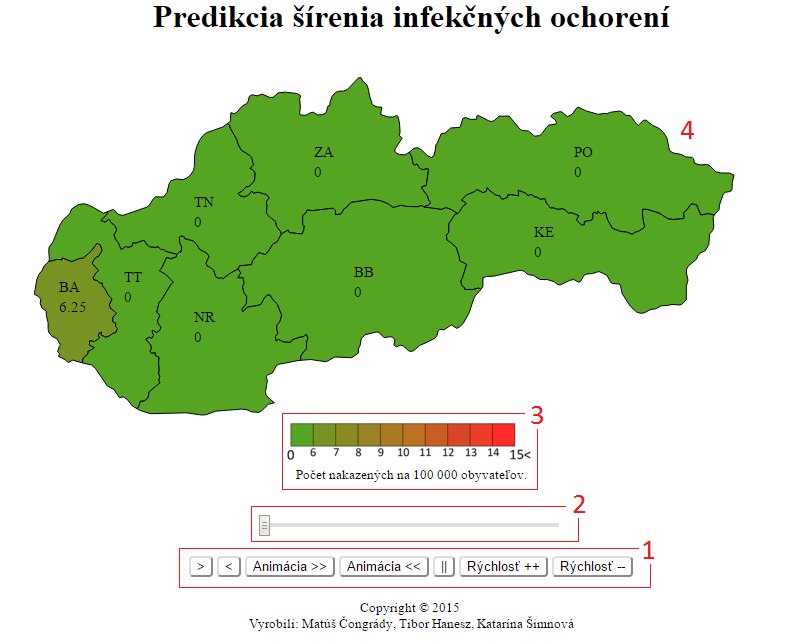
\includegraphics[scale=0.8]{front}
	\label{fig:front-end}
\end{figure}

\begin{itemize}
	\item 1 - Tato časť obsahuje funkcie pre manipuláciu s mapou. Zľava sú to:
		\begin{itemize}
			\item posunutie animácie o snímku vpred
			\item posunutie animácie o snímku vzad
			\item spustenie anímacie
			\item pretočenie animácie vzad
			\item pozastavenie animácie
			\item zrýchlenie animácie
			\item spomalenie animácie
		\end{itemize} 
	\item 2 - Slider pre lepšiu manipuláciu s animáciou. Rúčným posúvaním slidera je možné sledovať anímaciu v rôznych fázach.
	\item 3 - Legenda mapy. Farby krajov sa menia v závislosti od počtu nakazených v jednotlivých krajoch na 100 000 obyvateľov.
	\item 4 - Animácia šírenia infekčného ochorenie.
\end{itemize}

\renewcommand{\chaptername}{}	
\chapter[Administácia]{\rmfamily\bfseries
	Administácia}

\section{Prihlásenie}
\begin{figure}[htb]
	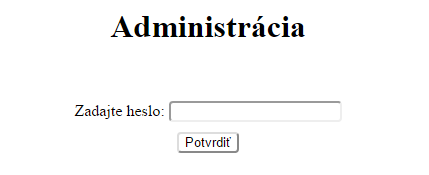
\includegraphics[scale=0.8]{prihlasenie}
	\label{fig:prihlasenie}
\end{figure}

\begin{itemize}

	\item Zadaním správneho hesla sa používateľ dostane do administácie
\end{itemize}

\pagebreak
\section{Nahranie súboru a zmena hesla}
\begin{figure}[htb]
	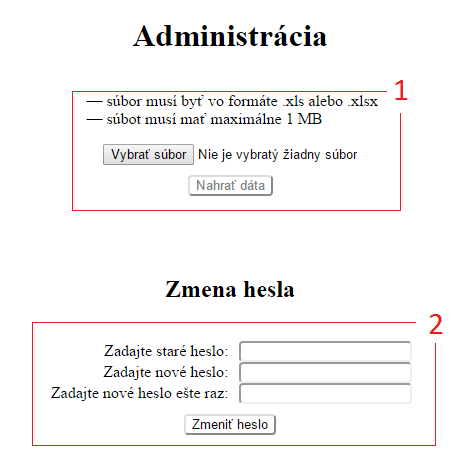
\includegraphics[scale=0.8]{administracia}
	\label{fig:administracia}
\end{figure}

\begin{itemize}
	\item 1 - Možnosť nahrať vstupny súbor vo formáte .xls alebo .xlsx
	\item 2 - Možnosť zmeny hesla
\end{itemize}
\pagebreak


\section{Tvar vstupnáho súboru}
\begin{figure}[htb]
	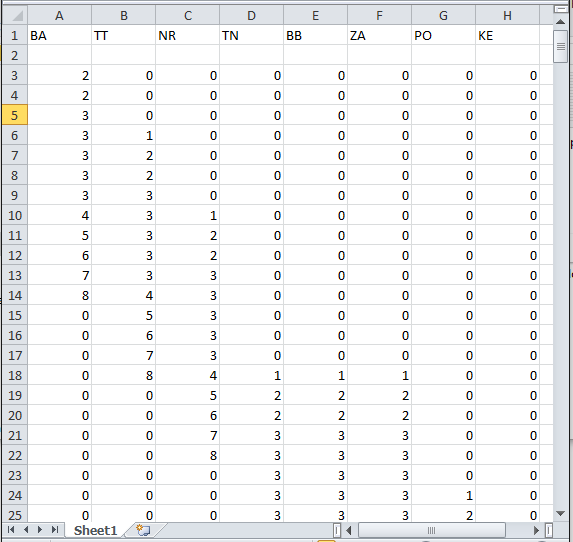
\includegraphics[scale=0.8]{vstup}
	\label{fig:vstup}
\end{figure}

\par Vstupom je tabuľka s ôsmimi stĺplcami, každý prislúcha jednemu kraju. V každom riadku sú hodnoty nakazených pre jeden deň. Číselné hodnoty udávajú absolútny počet nakazených v jednotlivých krajoch.

\end{document}